%%%%%%%%%%%%%%%%%%%%%%%%%%%%%%%%%%%%%%%%%%%%%%%%%%%%%%
\xchapter{Desenvolvimento}{Um breve resumo deste capítulo}
\label{cap:desenvolvimento}
%%%%%%%%%%%%%%%%%%%%%%%%%%%%%%%%%%%%%%%%%%%%%%%%%%%%%%


\section{Coleta e Análise de Dados} \label{analise} \textbf{ }
% Apresentar dados, gráficos e estudos de caso

    \citeonline{cohn2004user} descreve as seguintes técnicas para criação de um conjunto de histórias:
    \begin{itemize}
        \item Entrevistas com usuários;
        \item Questionários;
        \item Observação;
        \item Oficinas de redação de histórias.
    \end{itemize}

    Este trabalho utilizou-se de entrevistas com usuários reais para a construção do protótipo funcional.


\section{Implementação da Solução} \label{implement} \textbf{ }
% Apresentar o sistema neste capítulo

    \subsection{Apresentação do Software e das Tecnologias utilizadas} \textbf{ }

    \clearpage
    \subsection{Funcionalidades} \textbf{ }

        %Exemplo de tabela
        a Tabela \ref{tab:classification-of-gof-patterns} traz o detalhamento do ...
        
        \begin{table}[ht] 
        \caption{Classificação dos padrões de projeto GOF.}
        \label{tab:classification-of-gof-patterns}
        \begin{tabular*}{1\columnwidth}{@{\extracolsep{\fill}}>{\raggedright}p{0.25\columnwidth}>{\raggedright}p{0.75\columnwidth}}
        \toprule 
        \textbf{Element} & \textbf{Description}\tabularnewline
        \midrule
        \midrule 
        Patterns & Top element of the schema.\\It represents a collection of\\types of patterns\tabularnewline
        \midrule 
        Structurals & The set of Design Patterns classified as structural.\\Example: Decorator\\Design Pattern\tabularnewline
        \midrule 
        Behaviourals & The set of Design Patterns classified as creational.\\Example: Observer\\Design Pattern\tabularnewline
        \midrule 
        Creationals & The set of Design Patterns classified as behavioral.\\Example: Singleton\\Design Pattern\tabularnewline
        \midrule 
        \bottomrule
        \end{tabular*}
        \centering \\Fonte: Autores, 2024.
        \end{table}

            
    \clearpage
    
    \subsection{Imagens do Uso do Software} \textbf{ }

        % Exemplo de explicação de figura no texto
        A Figura \ref{fig:ifba-euc} mostra a imagem do Campus Euclides da Cunha.

        % Exemplo de inserção de figura no texto
        % A tabela de figura é atualizada automáticamente
        \begin{figure}[ht]
            \fontsize{12pt}{12pt}\selectfont
            \caption{IFBA - Campus Euclides da Cunha}
            \label{fig:ifba-euc}
            
            \centering
            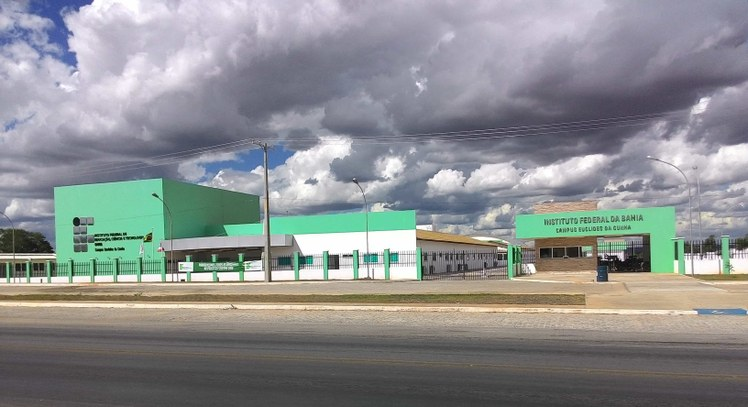
\includegraphics[scale=0.5]{imagens/ifba_euc.jpeg}
            \begingroup
                \fontsize{10pt}{10pt}\selectfont
                \centering \\Fonte: Autores, 2024.
            \endgroup
        \end{figure}  

        \clearpage
        Exemplo de algoritmo \ref{alg:BA}.
        \begin{algorithm}[ht]\label{alg:BA}
        \caption{\textit{Baseline Algorithm} (BA)}
        \small
        \KwIn{$Q=\{Q.D, Q.A, Q.T\}$}
        $R \leftarrow \emptyset$ \\
        \For{\textbf{each} $p \in P$}{ 
        	$containsAllTerms = \textit{true}$\\
        	\For{\textbf{each} $d \in Q.D$}{
        		$containsTerm = false$\\
        		\For{\textbf{each} $d' \in p.D$}{
        			\If{$d' = d$}{
        				$containsTerm = \textit{true}$
        			}
        		}
        		\If{\textbf{not} $containsTerms$}{
        			$containsAllTerms = false$
        		}
        	}
        	\If{$containsAllTerms$}{
        		\If{$Q.A_{1x} \leq p.x < Q.A_{2x}$ \textbf{and} $Q.A_{1y} \leq p.y \leq Q.A_{2y}$}{
        		\If{$Q.T_{1} \leq p.T \leq Q.T_{2}$}{
        			$R \leftarrow R \cup p$
        			}
        		}
        	}
        }
        \textbf{return} $R$
        \end{algorithm} 